% This is samplepaper.tex, a sample chapter demonstrating the
% LLNCS macro package for Springer Computer Science proceedings;
% Version 2.20 of 2017/10/04
%
\documentclass[runningheads]{llncs}
%
\usepackage{graphicx}
\usepackage{color}
\usepackage{amsmath}
\usepackage{amssymb}
\usepackage{bcprules, proof}
\usepackage{fancybox}
\usepackage{mathtools}
\usepackage{float}
\usepackage{xparse}
\usepackage{ebproof}
\usepackage{lscape}
\usepackage{mdframed}

% Used for displaying a sample figure. If possible, figure files should
% be included in EPS format.
%
% If you use the hyperref package, please uncomment the following line
% to display URLs in blue roman font according to Springer's eBook style:
% \renewcommand\UrlFont{\color{blue}\rmfamily}

\newcommand{\red}[1]{\textcolor{red}{#1 }}
\newcommand{\blue}[1]{\textcolor{blue}{#1 }}

\newcommand{\LTP}{$\lambda^{\triangleright\%}$}
\newcommand{\LMD}{$\lambda^{\textrm{MD}}$}
\newcommand{\LLF}{$\lambda^{\textrm{LF}}$}

\newcommand{\G}{\Gamma}
\newcommand{\D}{\Delta}
\newcommand{\V}{\vdash}
\newcommand{\VT}{\vdash\hspace{-.50em}\raisebox{0.28em}{\tiny{$\TB$}}}
\newcommand{\iskind}{\text{\ kind}}
\newcommand{\TW}{\triangleright}
\newcommand{\TWL}{\triangleleft}
\newcommand{\F}{\forall}
\newcommand{\TB}{\blacktriangleright}
\newcommand{\TBL}{\blacktriangleleft}
\newcommand{\E}{\equiv}
\newcommand{\FV}{\text{FV}}
\newcommand{\FTV}{\text{FTV}}

\newcommand{\WStar}{\textsc{W-Star}}
\newcommand{\WAbs}{\textsc{W-Abs}}
\newcommand{\WCsp}{\textsc{W-Csp}}
\newcommand{\WApp}{\textsc{W-App}}
\newcommand{\WTW}{\textsc{W-$\TW$}}

\newcommand{\KVar}{\textsc{K-Var}}
\newcommand{\KAbs}{\textsc{K-Abs}}
\newcommand{\KApp}{\textsc{K-App}}
\newcommand{\KConv}{\textsc{K-Conv}}
\newcommand{\KTW}{\textsc{K-$\TW$}}
\newcommand{\KTWL}{\textsc{K-$\TWL$}}
\newcommand{\KGen}{\textsc{K-Gen}}
\newcommand{\KCsp}{\textsc{K-Csp}}

\newcommand{\TVar}{\textsc{T-Var}}
\newcommand{\TAbs}{\textsc{T-Abs}}
\newcommand{\TApp}{\textsc{T-App}}
\newcommand{\TConv}{\textsc{T-Conv}}
\newcommand{\TTB}{\textsc{T-$\TB$}}
\newcommand{\TTBL}{\textsc{T-$\TBL$}}
\newcommand{\TGen}{\textsc{T-Gen}}
\newcommand{\TIns}{\textsc{T-Ins}}
\newcommand{\TCsp}{\textsc{T-Csp}}

\newcommand{\QKAbs}{\textsc{QK-Abs}}
\newcommand{\QKCsp}{\textsc{QK-Csp}}
\newcommand{\QKRefl}{\textsc{QK-Refl}}
\newcommand{\QKSym}{\textsc{QK-Sym}}
\newcommand{\QKTrans}{\textsc{QK-Trans}}

\newcommand{\QTAbs}{\textsc{QT-Abs}}
\newcommand{\QTApp}{\textsc{QT-App}}
\newcommand{\QTTW}{\textsc{QT-$\TW$}}
\newcommand{\QTGen}{\textsc{QT-Gen}}
\newcommand{\QTCsp}{\textsc{QT-Csp}}
\newcommand{\QTRefl}{\textsc{QT-Refl}}
\newcommand{\QTSym}{\textsc{QT-Sym}}
\newcommand{\QTTrans}{\textsc{QT-Trans}}

\newcommand{\QAbs}{\textsc{Q-Abs}}
\newcommand{\QApp}{\textsc{Q-App}}
\newcommand{\QTB}{\textsc{Q-$\TB$}}
\newcommand{\QTBL}{\textsc{Q-$\TBL$}}
\newcommand{\QGen}{\textsc{Q-Gen}}
\newcommand{\QIns}{\textsc{Q-Ins}}
\newcommand{\QCsp}{\textsc{Q-Csp}}
\newcommand{\QRefl}{\textsc{Q-Refl}}
\newcommand{\QSym}{\textsc{Q-Sym}}
\newcommand{\QTrans}{\textsc{Q-Trans}}
\newcommand{\QBeta}{\textsc{Q-$\beta$}}
\newcommand{\QEta}{\textsc{Q-$\eta$}}
\newcommand{\QTBLTB}{\textsc{Q-$\TBL\TB$}}
\newcommand{\QLambda}{\textsc{Q-$\Lambda$}}
\newcommand{\QPercent}{\textsc{Q-\%}}

\newcommand{\ID}[1]{\infer[]{#1}{\vdots}}
\newcommand{\MD}[1]{\mathcal{D}_#1}

\begin{document}
%
\title{A Dependently Typed Multi-Stage Calculus\thanks{Supported by organization x.}}
%
%\titlerunning{Abbreviated paper title}
% If the paper title is too long for the running head, you can set
% an abbreviated paper title here
%
\author{Akira Kawata\inst{1} \and
Atsushi Igarashi\inst{2}\orcidID{0000-0002-5143-9764}}
%
\authorrunning{A. Kawata, A. Igarashi}
% First names are abbreviated in the running head.
% If there are more than two authors, 'et al.' is used.
%
\institute{Graduate School of Informatics, Kyoto University, Kyoto, Japan\\
\email{akira@fos.kuis.kyoto-u.ac.jp} \and
\email{igarashi@kuis.kyoto-u.ac.jp}
}
%
\maketitle              % typeset the header of the contribution
%
\begin{abstract}


We develop yet another typed multi-stage calculus \LMD.
It extends Hanada and Igarashi's \LTP with dependent types.

A multi-stage calculus enables us to generate and execute codes at runtime.
It can improve the performance of programs by generating optimized codes for given inputs.

Dependent types are types dependent on values. 
Vectors with lengths are a famous example of dependent types and they enable us to omit boundary checking.

In this paper, we design \LMD by introducing dependent type into $\lambda^{\TW\%}$.
You can make more efficient programs from existing dependent typed programs with \LMD.

It has a simple, substitution-based full-reduction semantics and enjoys basic properties of subject reduction, confluence, and strong normalization, and progress.
It also includes an evaluation context which satisfies unique decomposition.

The main technical points of this paper are how to deal with Cross Stage Persistence of multi-stage calculuses which allows using a value in quoted code in a dependent type system.

The first point is CSP in kinding rules.
$\lambda^{\TW\%}$ includes kinding rules because dependent types need them
but the relationship between kinds and stages wasn't clear.

The second point is CSP in equivalence rules.
Parameters of dependent types may contain cross-staged terms.
We give reasonable equivalence rules to handle them.

\keywords{Multistage programming \and Dependent type}
\end{abstract}

\blue{213 words. The abstract should briefly summarize the contents of the paper in 150--250 words.}
%
%
%
\section{Introduction}
\subsection{Multi-Stage Calculus}
\subsubsection{Introduction to Multi-Stage Calculus}
\subsubsection{Application to Performance Imporving}
\subsection{Dependent Types}
\subsubsection{Introduction to Dependent Types}
\subsubsection{Application to Omitting Boundary Checking}
\subsection{Organaization of the Paper}

\section{Informal Overview of \LMD}
\subsection{\LLF}
\subsection{\LTP}
\subsection{\LMD}

\section{Formal Definition of \LMD}
\subsection{Syntax}

\begin{align*}
    \textrm{Terms} && M,N,L,O,P & ::= x \mid \lambda x:\tau.M\ \mid M\ M \mid \TB_\alpha M 
    \mid \TBL_\alpha M \mid \Lambda\alpha.M \mid M\ \epsilon \mid \%_\alpha M\\ 
    \textrm{Types} && \tau,\sigma,\rho,\pi,\xi & ::= X \mid \Pi x:\tau.\tau \mid \tau\ M \mid \TW_{\alpha} M \mid \F\alpha.\tau \\
    \textrm{Kinds} && K,J,I,H,G & ::= * \mid \Pi x:\tau.K\\
    \textrm{Contexts} && \Gamma & ::= \phi \mid 
    \Gamma,x:\tau @A\ (x\not\in\textrm{FV}(\G)) \mid 
    \Gamma,X::K @A\ (X\not\in \textrm{FV}(\G))\\
    \textrm{Transition variables} && & \alpha,\beta,\gamma, \dots \\
    \textrm{Transition} && & A,B,C,\dots \\
    \textrm{Variables} && & x,y,z,\dots \\
    \textrm{Type variables} && & X,Y,Z,\dots \\
\end{align*}

\subsection{Reduction}

\begin{definition}[Reduction]
\begin{align*}
    & (\lambda x:\tau.M) N \longrightarrow_\beta M[x \mapsto N] \\
    % & (\Pi x:\tau.\sigma) M \longrightarrow_\gamma \sigma[x \mapsto M] \\
    & \TBL_\alpha (\TB_\alpha M)\longrightarrow_\blacklozenge M \\
    & (\Lambda \alpha.M) \epsilon \longrightarrow_\Lambda M[\alpha \mapsto \epsilon]
\end{align*}
And take a minimum compatible relationship on terms.

    $ M \longrightarrow M'$ iff 
    $ M \longrightarrow_\Lambda M' $, $ M \longrightarrow_\blacklozenge M' $ or $ M \longrightarrow_\beta M' $.
\end{definition}

\subsection{Type System}
\subsubsection{Equivalence Rules}

\begin{definition}[Values]
$A \neq \epsilon$\\
\begin{align*}
    \textrm{Values} && v^\epsilon \in V^\epsilon & ::= \lambda x:\tau.M \mid\ \TB_\alpha v^\alpha \mid \Lambda\alpha.v^\epsilon & \\
                    && v^A \in V^A & ::= x \mid \lambda x:\tau.v^A \mid v^A\ v^A \mid\ \TB_\alpha v^{A\alpha} 
                                           \mid \Lambda\alpha.v^A \mid v^A\ \epsilon &\\
                                    &&& \quad\   \mid\ \TBL_\alpha v^{A'} (\text{if } A'\alpha = A \text{and } A' \neq \epsilon) & \\
                                    &&& \quad\   \mid \%_\alpha v^{A'} (\text{if } A'\alpha = A) & \\
    \textrm{Redexes} && R^\epsilon & ::= (\lambda x:\tau.M)\ v^\epsilon \mid (\Lambda\alpha.v^\epsilon)\ \epsilon & \\
                     && R^\alpha & ::=\ \TBL_\alpha \TB_\alpha M & \\
\end{align*}
\end{definition}


\begin{definition}[Staged Reduction]
$A \neq \epsilon$\\
\begin{align*}
    E^A_\epsilon [(\lambda x:\tau.M)\ v^\epsilon] & \longrightarrow_s E^A_\epsilon[M[x\mapsto v^\epsilon]] \\
    E^A_\epsilon [(\Lambda\alpha.v^\epsilon)\ \epsilon] & \longrightarrow_s E^A_\epsilon[v^\epsilon[\alpha\mapsto \epsilon]] \\
    E^A_\alpha [\TBL_\alpha \TB_\alpha v^\alpha] & \longrightarrow_s E^A_\alpha[v^\alpha] \\
\end{align*}
\end{definition}

\begin{definition}[Evaluation Context]
$A \neq \epsilon$\\
\begin{align*}
    E^\epsilon_B \in ECtx^\epsilon_B & ::= \square\ (\text{if\ } B = \epsilon) \mid E^\epsilon_B\ M \mid v^e\ E^\epsilon_B
                                           \mid \TB_\alpha E^\alpha_B \mid \Lambda\alpha.E^\epsilon_B
                                           \mid E^\epsilon_B\ \epsilon  \\
    E^A_B \in ECtx^A_B & ::= \square\ (\text{if } A = B) \mid \lambda x:\tau.E^A_B \mid E^A_B\ M \mid v^A\ E^A_B
                                           \mid E^\epsilon_B \mid \TB_\alpha E^{A\alpha}_B
                                           \mid \TBL_\alpha E^{A'}_B \ (\text{where } A'\alpha = A) \\
                                           & \quad \mid \Lambda\alpha.E^\epsilon_B
                                           \mid E^A_B\ \epsilon \mid \%_\alpha\ E^{A'}_B \ (\text{where } A'\alpha = A)\\
\end{align*}
\end{definition}

\section{Properties of \LMD}

\begin{theorem}[Substituition Lemma for Variables of Terms, Types or Kinds and Their Equivalence]
    \begin{flalign*}
        \text{If\ } \G,z:\xi @B \V M:\tau @A \text{\ and\ } \G\V P:\xi @B
        &\text{\ then\ } \G\V M[z \mapsto P]:\tau[z \mapsto P] @A.&\\
        \text{If\ } \G,z:\xi @B \V \tau::K @A \text{\ and\ } \G\V P:\xi @B
        &\text{\ then\ } \G\V \tau[z \mapsto P]::K[z \mapsto P] @A.&\\
        \text{If\ } \G,z:\xi @B \V K\iskind @A \text{\ and\ } \G\V P:\xi @B
        &\text{\ then\ } \G\V K[z \mapsto P] \iskind  @A.&\\
        \text{If\ } \G,z:\xi @B \V M\E N : \tau @A \text{\ and\ } \G\V P:\xi @B
        &\text{\ then\ } \G\V M[z \mapsto P]\E N[z \mapsto P] : \tau[z \mapsto P] @A.&\\
        \text{If\ } \G,z:\xi @B \V \tau\E \sigma : K @A \text{\ and\ } \G\V P:\xi @B
        &\text{\ then\ } \G\V \tau[z \mapsto P]\E \sigma[z \mapsto P] : K[z \mapsto P] @A.&\\
        \text{If\ } \G,z:\xi @B \V K\E J @A \text{\ and\ } \G\V P:\xi @B
        &\text{\ then\ } \G\V K[z \mapsto P]\E J[z \mapsto P] @A.&
    \end{flalign*}    
\end{theorem}

\begin{theorem}[Stage Substituition Lemma for Variables of Terms, Types or Kinds and Their Equivalence]
    \begin{flalign*}
        \text{If\ } \G \V M:\tau @A
        &\text{\ then\ } \G[\beta \mapsto \epsilon]\V M[\beta \mapsto \epsilon]:\tau[\beta \mapsto \epsilon] @A[\beta \mapsto \epsilon].&\\
        \text{If\ } \G \V \tau::K @A
        &\text{\ then\ } \G[\beta \mapsto \epsilon]\V \tau[\beta \mapsto \epsilon]::K[\beta \mapsto \epsilon] @A[\beta \mapsto \epsilon].&\\
        \text{If\ } \G \V K\iskind @A
        &\text{\ then\ } \G[\beta \mapsto \epsilon]\V K[\beta \mapsto \epsilon] \iskind @A[\beta \mapsto \epsilon].&\\
        \text{If\ } \G \V M\E N : \tau @A
        &\text{\ then\ } \G[\beta \mapsto \epsilon]\V M[\beta \mapsto \epsilon]\E N[\beta \mapsto \epsilon] : \tau[\beta \mapsto \epsilon]  @A[\beta \mapsto \epsilon].&\\
        \text{If\ } \G \V \tau\E \sigma : K @A
        &\text{\ then\ } \G[\beta \mapsto \epsilon]\V \tau[\beta \mapsto \epsilon]\E \sigma[\beta \mapsto \epsilon] : K[\beta \mapsto \epsilon] @A[\beta \mapsto \epsilon].&\\
        \text{If\ } \G \V K\E J @A
        &\text{\ then\ } \G[\beta \mapsto \epsilon]\V K[\beta \mapsto \epsilon]\E J[\beta \mapsto \epsilon] @A[\beta \mapsto \epsilon].&
    \end{flalign*}
\end{theorem}

\begin{theorem}[Preservation for term on $\beta$ reduction]
    If $\G\V M:\tau @A$ and $M \longrightarrow_{\beta} M'$, then $\G\V M':\tau @A$\\
\end{theorem}

\begin{theorem}[Preservation for term on $\TBL\TB$ reduction]
    If $\G\V M:\tau @A$ and $M\longrightarrow_\blacklozenge N$, then $\G\V N:\tau @A$\\
\end{theorem}

\begin{theorem}[Preservation for term on $\Lambda$ reduction]
    If $\G\V M:\tau @A$ and $M \longrightarrow_{\Lambda} N$, then $\G\V N:\tau @A$.
\end{theorem}

\begin{theorem}[Strong Normalization]
    If $\G\V^A t:T$ then there is no infinite sequence of terms $(t_i)_{i\ge1}$ and $t_i \longrightarrow_{\beta, \TBL \TB,\Lambda} t_{i+1}$ for $i\ge 1$
\end{theorem}

\begin{theorem}[Confluence(Church-Rosser Property)]
    Define $M \longrightarrow N$ as $M \longrightarrow_{\beta} N$ or $M\longrightarrow_\blacklozenge N$ or  $M \longrightarrow_{\Lambda} N$.\\
    For any term $M$, if $M \longrightarrow^* N$ and $M \longrightarrow^* L$,
    there exists $O$ that satisfies $N \longrightarrow^* O$ and $L \longrightarrow^* O$.
\end{theorem}

\begin{theorem}[Progress]
    If $x:\tau @\epsilon \notin \G$ and $\G \V M : \tau  @ A$ then $ M \in V^A $ or $\exists M'$ such that $M \longrightarrow M'$.
\end{theorem}

\begin{theorem}[Unique Decomposition]
    If $x:\tau@\epsilon \notin \G$ and $\G \V M : \tau @ A$ then 1 or 2 is true.
    \begin{enumerate}
        \item $ M \in V^A$
        \item $\exists ! B, E^A_B, R^B$ such that ($B = \epsilon$ or $B = \beta$) and $M = E^A_B[R^B]$.
    \end{enumerate}
\end{theorem}

\section{Related Work}

\begin{itemize}
   \item On Cross-Stage Persistence in Multi-Stage\cite{Hanada2014}

   CSPも入りました
   \item Eliminating Array Bound Checking Through Dependent Types\cite{Xi98}
   \item MetaML and Multi-stage Programming with Explicit Annotations\cite{MetaML}
   \item Idris, a general-purpose dependently typed programming language: Design and implementation\cite{brady2013idris}
   \item A Logical Foundation for Environment Classifiers\cite{Tsukada}
   \item Environment classifiers\cite{taha2003environment}
   \item A framework for defining logics\cite{harper1993framework}

    $\Sigma$ の使い方を確認した
   \item The Design and Implementation of {BER} MetaOCaml - System Description\cite{oleg2014}
   \item Refined Environment Classifiers\cite{kiselyov2016refined}
   \item Staging with control: type-safe multi-stage programming with control operators\cite{oishi2017staging}
   \item \red{Partial evaluation and automatic program generation}\cite{jones1993partial}
   \item \red{Efficient multi-level generating extensions for program specialization}\cite{gluck1995efficient}
   \item Dependent types in practical programming\cite{xi1999dependent}

        Section of Applicationを読んだ。Dead Code EliminationやLoop Unrollingにも使えるらしい。

   \item A dependently typed assembly language\cite{xi2001dependently}

   DTALの定義と制約solverを用いた型検査の定義
   \item \red{Run-time code generation and Modal-ML}\cite{wickline1998run}
   \item \red{C and tcc: a language and compiler for dynamic code generation}\cite{poletto1999c}
   \item \red{Run-time bytecode specialization}\cite{masuhara2001run}
   \item \red{A tour of Tempo: A program specializer for the C language}\cite{consel2004tour}
   \item \red{Optimizing ML with run-time code generation}\cite{lee1996optimizing}
   \item \red{Efficient incremental run-time specialization for free}\cite{marlet1999efficient}

\end{itemize}

\section{Conclusions}

% \section{First Section}
% \subsection{A Subsection Sample}
% Please note that the first paragraph of a section or subsection is
% not indented. The first paragraph that follows a table, figure,
% equation etc. does not need an indent, either.
% 
% Subsequent paragraphs, however, are indented.
% 
% \subsubsection{Sample Heading (Third Level)} Only two levels of
% headings should be numbered. Lower level headings remain unnumbered;
% they are formatted as run-in headings.
% 
% \paragraph{Sample Heading (Fourth Level)}
% The contribution should contain no more than four levels of
% headings. Table~\ref{tab1} gives a summary of all heading levels.
% 
% \begin{table}
% \caption{Table captions should be placed above the
% tables.}\label{tab1}
% \begin{tabular}{|l|l|l|}
% \hline
% Heading level &  Example & Font size and style\\
% \hline
% Title (centered) &  {\Large\bfseries Lecture Notes} & 14 point, bold\\
% 1st-level heading &  {\large\bfseries 1 Introduction} & 12 point, bold\\
% 2nd-level heading & {\bfseries 2.1 Printing Area} & 10 point, bold\\
% 3rd-level heading & {\bfseries Run-in Heading in Bold.} Text follows & 10 point, bold\\
% 4th-level heading & {\itshape Lowest Level Heading.} Text follows & 10 point, italic\\
% \hline
% \end{tabular}
% \end{table}
% 
% 
% \noindent Displayed equations are centered and set on a separate
% line.
% \begin{equation}
% x + y = z
% \end{equation}
% Please try to avoid rasterized images for line-art diagrams and
% schemas. Whenever possible, use vector graphics instead (see
% Fig.~\ref{fig1}).
% 
% \begin{figure}
% 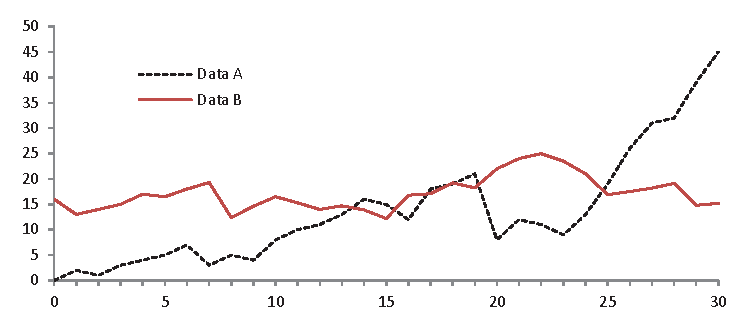
\includegraphics[width=\textwidth]{fig1.eps}
% \caption{A figure caption is always placed below the illustration.
% Please note that short captions are centered, while long ones are
% justified by the macro package automatically.} \label{fig1}
% \end{figure}
% 
% \begin{theorem}
% This is a sample theorem. The run-in heading is set in bold, while
% the following text appears in italics. Definitions, lemmas,
% propositions, and corollaries are styled the same way.
% \end{theorem}
% %
% % the environments 'definition', 'lemma', 'proposition', 'corollary',
% % 'remark', and 'example' are defined in the LLNCS documentclass as well.
% %
% \begin{proof}
% Proofs, examples, and remarks have the initial word in italics,
% while the following text appears in normal font.
% \end{proof}
% For citations of references, we prefer the use of square brackets
% and consecutive numbers. Citations using labels or the author/year
% convention are also acceptable. The following bibliography provides
% a sample reference list with entries for journal
% articles~\cite{ref_article1}, an LNCS chapter~\cite{ref_lncs1}, a
% book~\cite{ref_book1}, proceedings without editors~\cite{ref_proc1},
% and a homepage~\cite{ref_url1}. Multiple citations are grouped
% \cite{ref_article1,ref_lncs1,ref_book1},
% \cite{ref_article1,ref_book1,ref_proc1,ref_url1}.
%
% ---- Bibliography ----
%
% BibTeX users should specify bibliography style 'splncs04'.
% References will then be sorted and formatted in the correct style.
%
\bibliographystyle{splncs04}
\bibliography{main}
%
% \begin{thebibliography}{8}
% \bibitem{ref_article1}
% Author, F.: Article title. Journal \textbf{2}(5), 99--110 (2016)
% 
% \bibitem{ref_lncs1}
% Author, F., Author, S.: Title of a proceedings paper. In: Editor,
% F., Editor, S. (eds.) CONFERENCE 2016, LNCS, vol. 9999, pp. 1--13.
% Springer, Heidelberg (2016). \doi{10.10007/1234567890}
% 
% \bibitem{ref_book1}
% Author, F., Author, S., Author, T.: Book title. 2nd edn. Publisher,
% Location (1999)
% 
% \bibitem{ref_proc1}
% Author, A.-B.: Contribution title. In: 9th International Proceedings
% on Proceedings, pp. 1--2. Publisher, Location (2010)
% 
% \bibitem{ref_url1}
% LNCS Homepage, \url{http://www.springer.com/lncs}. Last accessed 4
% Oct 2017
% \end{thebibliography}

\blue{We solicit submissions in the form of regular research papers describing original scientific research results, including system development and case studies. Regular research papers should not exceed 18 pages in the Springer LNCS format, including bibliography and figures. This category encompasses both theoretical and implementation (also known as system descriptions) papers. In either case, submissions should clearly identify what has been accomplished and why it is significant. Submissions will be judged on the basis of significance, relevance, correctness, originality, and clarity. System descriptions papers should contain a link to a working system and will be judged on originality, usefulness, and design. In case of lack of space, proofs, experimental results, or any information supporting the technical results of the paper could be provided as an appendix or a link to a web page, but reviewers are not obliged to read them.}
\end{document}
